
\section{Deferred Tessellation}


\label{sec:tessellation}
%After intersection computation, tessellation is performed on each intersecting triangle face to generate the intersection-free meshes. We call this step as deferred tessellation because the tessellation happens until all valid intersections are computed, instead of clipping triangle incrementally by each intersection.

After intersection computation, tessellation is performed on each intersecting triangle face to generate the intersection-free meshes. This step is referred to as deferred tessellation, because the tessellation happens after all of the valid intersections are computed, instead of clipping triangles incrementally at each intersection.

%Ogayar-Anguita et. al. \cite{ogayar2015deferred} use Constrained Delaunay Triangulation (CDT) to perform deferred tessellation. They treat triangle faces as convex triangulation zones and intersections as constraints. Our first try is to implement a robust plane-based CDT. However, CDT algorithms \cite{chew1989constrained,preparata2012computational} require coordinates projection or intersection detection between arbitrary connections of vertices within triangulation zone, which are difficult to be implemented under P-reps. From another perspective, CDT contains geometry constructions---new edges are generated to guarantee each subface is a triangle (see Fig. \ref{fig:iisect}d), which is not preferred in our method. Moreover, when there are more than two primitives, simply applying CDT omits the complexity of intersections between meshes---the intersections may intersect each other, introducing new vertices and splitting original intersection line segments (see Fig. \ref{fig:iisect}a). This breaks the assumption of most CDT algorithms and may lead to incorrect output topology.

Ogayar-Anguita et al. \cite{ogayar2015deferred} used CDT to perform deferred tessellation. They treated triangle faces as convex triangulation zones, and intersections as constraints. We first attempted to implement robust plane-based CDT. However, CDT algorithms \cite{chew1989constrained,preparata2012computational} require the projection of coordinates, or intersection detection between arbitrary connections of vertices within the triangulation zone; both of which are difficult to implement using P-reps. Additionally, CDT produces geometric constructions��new edges are generated to guarantee that each subface is a triangle (see Fig. \ref{fig:iisect}d)��which we preferred not to use in our method. Moreover, when there are more than two primitives, applying CDT ignores the complexity of the intersections between meshes. For instance, the intersections may intersect each other, introducing new vertices and splitting the original intersecting line segments (see Fig. \ref{fig:iisect}a). This breaks the assumptions of most CDT algorithms, and may lead to incorrect output topologies.

\begin{figure}[t]
\centering
\includegraphics[width=3.5in]{boolean-04}
\caption{a) Different colors indicate that the intersections originate from different meshes. The yellow and red intersections intersect at a point. The yellow intersection overlaps with the green intersection. b) After refinement, we introduce a new vertex $\bm{v}_a$, and merge overlapping intersections into a single edge $\bm{e}_b$. c) Our tessellation method does not guarantee that all of the faces are triangular. d) If triangulation is performed, new edges (red lines) are introduced and precise plane-based representations cannot be constructed for these new edges.}
%a) Different colors indicate the intersections are from different meshes. The yellow intersection and the red intersection intersect at a point. Also, the yellow intersection overlap with the green intersection. b) After refinement, we introduce a new vertex $\bm{v}_a$, and merge overlapping intersections into one edge $\bm{e}_b$. c) Our tessellation does not guarantee to obtain triangles. d) If triangulation is performed, new edges (red lines) are introduced and we cannot give the precise plane-based representation for these new edges.
\label{fig:iisect}
\end{figure}

%To solve these problems, we first perform intersection refinement to eliminate any crossing or overlapping between intersections. After that, we perform conservative tessellation based on \emph{tess-graph}, ensuring unconditional topology correctness. An tess-graph is a graph-like description of intersections on a certain face. The word `conservative` means we do not add any new edge during tessellation, which do not guarantee the subfaces are triangles.

In our method we first perform intersection refinement to eliminate any crossing or overlapping between intersections. We then perform conservative tessellation based on a \emph{tess-graph}, ensuring unconditional topologic correctness. A tess-graph is a graph-like description of the intersections on a given face. The word 'conservative' in this instance means that we do not add any new edges during tessellation, which does not guarantee that the subfaces are all triangular.

\subsection{Intersection Refinement}

\label{sec:refine}
%The intersection vertices are not only introduced by intersection between an edge and a triangle, but also introduced by intersections of three triangles. In order to find all intersection vertices, it is not enough by only triangle-triangle intersection tests. Thus, we have to refine these triangle-triangle intersections before the real tessellation.

Intersection vertices can be introduced by the intersection of three triangles, in addition to intersections between an edge and a triangle. Triangle-triangle intersection tests alone are not sufficient to determine all of the intersection vertices. Thus, it is necessary to refine these triangle-triangle intersections before the final tessellation.

Intersection refinement is performed in locally. For each intersecting face $t$, we collect all of the intersections on $t$ as a set $\bm{\Gamma}(t)$ and refine them as a set. We also include the three edges of $t$ in $\bm{\Gamma}(t)$, because the edges also participate in tessellation. In $\bm{\Gamma}(t)$, edges are represented as PBIs. The neighborhood $\mathcal{N}$ of the edges are set as $N/A$ because they do not have a neighborhood. Other PBI-rep components can be determined by the P-reps of the edges. The refinement of $\bm{\Gamma}(t)$ is done using only plane-based geometric predicates, in the following three steps.


\vspace{0.5em}
\noindent \textbf{Coincidence elimination}~~~~
%We merge coincidence intersections which have the same end points. Intersections are undirected so intersections with inverse end points are also coincident. The PBI-rep of the merging intersection is inherited from either of the old one's except the neighborhood component. The new neighborhood is the union of the merged ones', meaning the intersection has two (or more) neighborhoods.
We merge coincidence intersections that have the same end points. Intersections are undirected, so intersections with inverse end points are also coincident. The PBI-rep of the merged intersection is inherited from either of the original intersections, except for the neighborhood component of the PBI-rep. The new neighborhood component is the union of the original intersections�� components, meaning that the merged intersection has two (or more) neighborhoods.

\vspace{0.5em}
%Intersection refinement is performed locally
\begin{wrapfigure}{r}[0in]{0in}
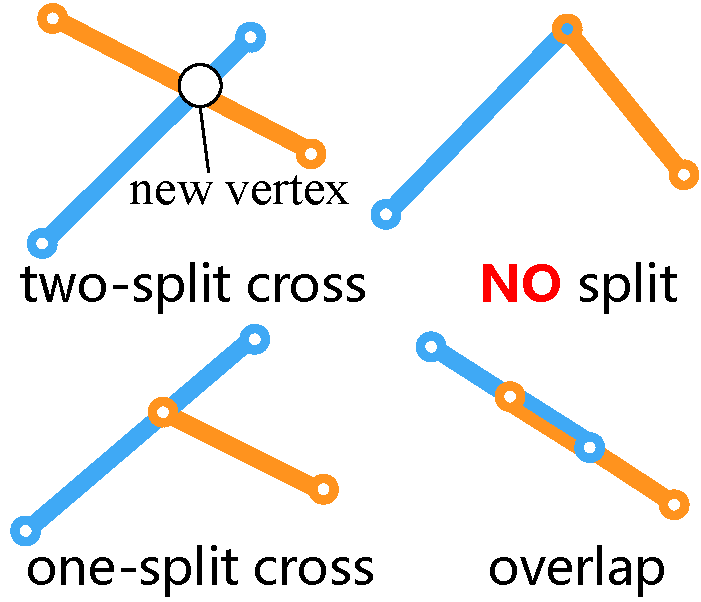
\includegraphics[width=1.6 in]{resolve}
%\caption{Plane-based representation of triangle}
\end{wrapfigure}
\noindent\textbf{Cross and overlap resolving}~~~~
%After the process of two previous steps, there are no overlapping intersections in $\bm{\Gamma}(t)$. We check whether any pair of intersections cross or overlap (collinear) each other. New vertices might be introduced in this step. The definition of \emph{cross} does not include the situation that two intersections share one end point, since no splitting is required in this situation. When there is crossing or overlapping, at least one of the intersections have to be split. Because one intersection may may 'touch' more than one other intersections, the splitting is deferred until all splitting points are found. The subroutine linear order of points (\S\ref{sec:substrates}) is used to sort these splitting points along the splitting intersection. The PBI-reps of split segments inherit their father's except the $\bm{P}_0, \bm{P}_1$, which identifies the P-reps of end points*.
After the two previous steps, there are no overlapping intersections remaining in $\bm{\Gamma}(t)$. We then check whether any pair of intersections cross or overlap (are collinear to) each other. New vertices can be introduced in this step. The definition of \emph{cross} does not include the situation where two intersections share a single end point because no splitting is required in this situation. When there is crossing or overlapping, at least one of the intersections has to be split. Because one intersection may be in contact with more than one other intersection, this splitting is deferred until all of the splitting points are found. The subroutine for determining the linear order of the points (\S\ref{sec:substrates}) is used to sort these splitting points along the splitting intersection. The PBI-reps of the split segments inherit that of their father��s, except for $\bm{P}_0, \bm{P}_1$, which identifies the P-reps of the end points*.

\vspace{0.5em}
\noindent \textbf{Coincidence elimination (revisited)}~~~~
%Unfortunately, the overlap resolving may bring new coincident intersections in overlap cases. Therefore the first step is run again in the final step.
Unfortunately, resolving the overlap may produce new coincident intersections. Therefore, the first step of the process is repeated in the final step.

\subsection{Tessellation by Tess-Graph}
\label{sec:tess}



%So far, intersections are only independent data that store the coordinates and neighbourhood information. To perform tessellation and extract subfaces, we need to organize them to reveal the topology. We use tess-graph for this purpose. A tess-graph is the graph description of the tessellated face topology. For each face to be tessellated, we construct a tess-graph according to the refined intersections. Nodes of tess-graph represent end points of intersections and undirectional connections between nodes represent intersections. The construction of tess-graph is straightforward and the reader will not have problem filling the details.

Intersections are independent data that store coordinates and neighborhood information. To perform tessellation and extract subfaces, we need to organize them to determine topology. We use a tess-graph for this purpose. A tess-graph is the graph description of the tessellated face topology. For each face to be tessellated, we construct a tess-graph from the refined set of intersections. Nodes of the tess-graph represent the end points of intersections, and nondirectional connections between nodes represent intersections. The construction of a tess-graph is straightforward, and readers should be able to determine the details.

%After we have tess-graph, we tessellate face and extract subfaces according to it. This is done by extract valid loops on tess-graph. A valid loop must satisfy two criterions: 1) the direction of loops should be coherent with the face normal, and 2) consecutive connections on the loop should be adjacent by circular order. Each valid loop corresponds to a intersection-free face. After we find out all valid loops on tess-graph, we finish tessellating the corresponding face (see Fig. \ref{fig:cadj}). To facilitate the later process, we also store neighborhood information into the edges of the new faces. The neighborhood information is inherent from the corresponding intersections. When all faces are tessellated, meshes are intersection-free.

After the tess-graph is constructed, we tessellate the face and extract subfaces from it. Subfaces are extracted from valid loops on the tess-graph. A valid loop must satisfy two criteria: 1) the direction of the loop should correspond with the face normal, and 2) consecutive connections on the loop should be adjacent by circular order. Each valid loop corresponds to an intersection-free face. After all of the valid loops are determined from the tess-graph, the corresponding face is tessellated (Fig. \ref{fig:cadj}). To facilitate later processes, we also store neighborhood information in the edges of the new faces. The neighborhood information is determined from the corresponding intersections. When all faces are tessellated, the corresponding meshes are intersection-free.

\begin{figure}[t]
\centering
\includegraphics[width=3in]{boolean-05}
\caption{a) To tessellate a triangle, we find all of the valid loops on a tess-graph. The direction of the loops must be coherent with the triangle normal (assuming here that the normal points to the outside of the paper). b) Each circular adjacent edge pair is an angle of the tessellated polygon.}
\label{fig:cadj}
\end{figure}
